%! TEX root = diss.tex
\documentclass[../diss.tex]{subfiles}
\chapter{Implementation}

% NOTE: Multiprocessor => shared memory. Use term "parallel computer" instead

% Introduction:
% * TODO: change fig 2.1 to have cloud of "graph data.csv" that interact with
%   "input graph"
% * Refer to figure 2.1, go into some more depth on interface to Parallel
%   system simulation:
%   * You create Worker implementation with access to ...., then pass
%     description to manager, specify number of workers, topology to use, num
%     computation phases, etc.
% * _Intrdc the different components, and then start going into detail in ind. subsecs_
% * Figure of the repository overview goes here

% Repo overview figure
% Repostory overview figure {{{

\begin{figure}[htp]
\begin{center}
    \begin{adjustbox}{valign=t}
    \begin{forest}
        dirtree,
        [part-ii-project/
        [scripts/
            [graph-extractor.py]
            [download-spatial-datasets.sh]
            [random-graphs.py]
            [evaluation.py]
        ]
        [ParallelAPSP/src/
        [test/java/
            [$\dots$]
        ]
        [main/java/
        [APSPSolver/
            [\textit{APSPSolver.java}]
            [MatSquare.java]
            [SerialDijkstra.java]
        ]
        [graphReader/
            [GraphReader.java]
            [GraphCompressor.java]
        ]
        [main/
            [Evaluation.java]
        ]
        [matrixMultiplication/
            [BroadcastMatrix-\\{ }Multiplication.java]
            [FoxOtto.java]
            [GeneralisedFoxOtto.java]
            [\textit{MinPlusProduct.java}]
        ]
        [util/
        [LoggerFormatter.java]
        [Matrix.java]
        [Triple.java]
        ]
        [$\vdots$, dots]
        ]]]
    \end{forest}
\end{adjustbox}\qquad
\begin{adjustbox}{valign=t}
    \begin{forest}
        dirtree,
        [\,$\vdots$
        [memoryModel/
        [CommunicationChannel-\\{ }CongestionException.java]
        [CommunicationChannel-\\{ }Exception.java]
        [InconsistentCommunication-\\{ }ChannelUsageException.java]
        [CommunicationManager.java]
        [PrivateMemory.java]
        ]
            [timingAnalysis/
                [MultiprocessorAttributes.java]
                [Timed-\\{ }CommunicationManager.java]
                [TimedManager.java]
                [TimedMatSquare.java]
                [TimedWorker.java]
                [TimingAnalysisResult.java]
                [topology/
                    [\textit{Topology.java}]
                    [SquareGridTopology.java]
                ]
            ]
            [work/
                [Manager.java]
                [WorkerFactory.java]
                [WorkerInstatiationException.java]
                [\textit{Worker.java}]
                [WorkersFailedToComplete-\\{ }Exception.java]
            ]
        ]
    \end{forest}
\end{adjustbox}
\end{center}
\caption[Repository overview]{\textbf{Repository overview} Text in italics
    indicate Java interfaces or abstract classes.  Subdirectories within
    \texttt{main/java/}
    are Java packages. An overview of the unit tests in the \texttt{test/java/}
    directory is presented in \cref{sec:Unit tests} and their result
    in \cref{fig:unit-test-full}.
    The whole codebase, as presented here, contains 5880 lines of Java code,
    and 729 lines of Python code.  The \texttt{work/}, \texttt{memoryModel/}
    and \texttt{timingAnalysis/} packages are elaborated in their
    respective subsections in \cref{sec:Simulation of a distributed memory
    multiprocessor}, and the \texttt{APSPSolver/} and
    \texttt{matrixMultiplication/}
    packages are described in \cref{sec:APSP via repeated matrix-squaring}.
}
\label{fig:repo-overview}
\end{figure}

% }}}

This chapter elaborates on how the final codebase, as shown in
\cref{fig:repo-overview}, accomplishes all the requirements laid out in
\cref{sec:Requirements analysis}.
I start by covering the input graphs in \autoref{sec:Graph datasets}.
Afterwards, I explain how I simulated a parallel system
in \cref{sec:Simulation of a distributed memory multiprocessor}. The simulator
provides an expressive, yet simple, interface for writing and timing the execution
of massively parallel programs. In \cref{sec:APSP via repeated matrix-squaring},
this interface is used to implement the
\ac{MatSquare} algorithm, which is a massively parallel algorithm for solving
\ac{APSP}. Finally, I describe an optimisation to the algorithm in
\cref{sec:Graph compression}.

% Some "practices used/software dev.? chapter":
% * Weekly meetings, log book,

% Graph datasets:
% * California road networks:
%   * freely-available, consisten format, real-life road network
% * Random graphs:
%   * To satisyf req. of different n
%   * Erdos-Renyi graph, but modified to be fully-connected, trick to get same properties
%     with formula for creating $p$
%   *  python library used
% * Graph reader
%   * adjacency matrix and also neighbourhood list for Dijkstra's algorithm
% Graph datasets {{{
\section{Graph datasets}%
\label{sec:Graph datasets}

To run the algorithms, we need graphs as input. Since one important usage of \ac{APSP}
is route-planning, I used a dataset of the Californian road-network. This dataset was
initially presented by \citeauthor{graph-dataset} and has been made available on the author's
website\footnote{\url{https://www.cs.utah.edu/~lifeifei/SpatialDataset.htm}}
\cite{graph-dataset}.
This graph has 21048 vertices and will be used to prove that the
\ac{MatSquare} algorithm can efficiently solve practical
route-planning problems on a parallel system.
However, to evaluate the algorithm's scalability, I need graphs of a wide
range of different sizes. These were generated randomly.

\subsection{Random graph generation}%
\label{sub:Random graph generation}

% TODO: mention that fully connected because mimic road networks...

% TODO: information on Erdos-Renyi graphs in prepreration chapter...


To generate the graphs,
I used \erdos graphs, specifically the $G(n,p)$ model:
We start with an edge-less graph of
$n$ vertices. We then independently include each of
the $n^2$ edges with probability $p$. I chose this model because it allows
specifying the graph's size, and it has previously
been used to evaluate the performance of \ac{APSP} algorithms
\cite{parallelDijkstra}.
% TODO: cite https://core.ac.uk/download/pdf/81103122.pdf
%            https://www.researchgate.net/publication/47842024_A_Parallelization_of_Dijkstra%27s_Shortest_Path_Algorithm

\subsubsection{Choice of parameter $p$}%
\label{ssub:Choice of parameter $p$}

\begin{wraptable}{r}{0.46\textwidth}
    \vspace{-10pt}
    \centering
    \begin{tabular}{|m{0.28\textwidth}|m{0.11\textwidth}|}
        \hline
        \textbf{Location} & \textbf{Average vertex degree} \\
        \hline
        San-Francisco (SF) &  2.549 \\
        \hline
        North-America (NA) & 2.038 \\
        \hline
        City of Oldenburg (OL) & 2.305 \\
        \hline
        California (cal) & 2.061 \\
        \hline
        California (compressed) & 2.945 \\
        \hline
        City of San Joaquin (TG) & 2.614 \\
        \hline
    \end{tabular}%
    \caption[Average vertex degree of different road-network datasets]{Average vertex degree in various road-network datasets\footnotemark.}%
    \label{tab:vertex-degree}
    \vspace{-10pt}
\end{wraptable}

\footnotetext{These values were computed using the 
\texttt{printSummary} method in the \texttt{GraphReader} class.}

To allow the evaluation to better reason about the practicality of
\ac{MatSquare} for route-planning problems, we want the input graphs
to have matching characteristics to that of real-world graphs. With a clever choice of
$p$, we can achieve this.

There are many characteristics of a graph, such as vertex- and
edge-connectivity, betweenness centrality, and clustering coefficient. 
However, trying to generate new graphs with similar values for all
of these metrics is another project itself.  I have therefore only
tried to replicate the metric, \textit{average vertex degree}, which has
some correlation to these metrics. I also want the random graphs
to be connected, as most road-networks are. In the $G(n,p)$ random-graph
model, the number of edges follows the binomial distribution:
\begin{equation}
    \textrm{For vertex } v \in V, \;\;\textrm{deg}(v) \sim \textrm{Binomial}(n-1,p),
\end{equation}
with the average degree being $(n-1)p$. By modifying the graph generation
algorithm to start with a
\textit{circular graph}%
\footnote{Each vertex has exactly 2 neighbours.},
and including each remaining edge independently with probability
\begin{equation}
    p=\frac{\textrm{desired average degree} - 2}{n - 3},
\end{equation}
we get a connected graph where the average degree is as desired. We can then
sample the edge-weights from the uniform distribution to get a weighted graph.

I chose the desired average degree based on that of 
the Californian road-network. 
However, since we will be using the compressed graph (see
\autoref{sec:Graph compression}), I used the average vertex degree of the
compressed California graph instead, which was 2.945. In
\autoref{fig:example-graph-random}, I have plotted an example graph generated
through this method. I then generated 22 graphs of various sizes for use
in evaluation%
\footnote{To get a sense of scaling for both small and large problem sizes,
the graphs were of sizes: \texttt{10,20,30,40,50,60,70,80,90,100,%
150,200,250,300,350,400,450,500,550,600,650}, and \texttt{700}.}.

\begin{figure}
\begin{center}
    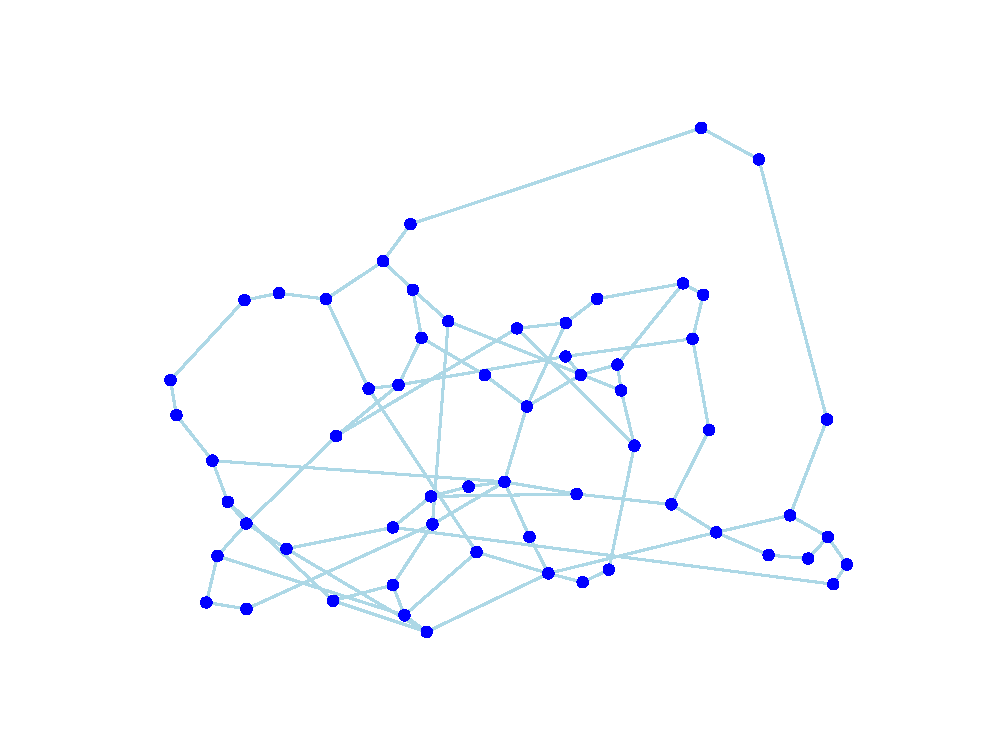
\includegraphics[scale=.7]{figs/plots/example-graph.eps}
\end{center}
\caption[Example of \erdos graph]{A visualisation of a graph generated with the modified
\erdos model. The graph has $n=60$ vertices, and the length of the
edges correspond to their weight\footnotemark.}%
\label{fig:example-graph-random}%
\end{figure}

\footnotetext{The graph was visualised using the \texttt{ForceAtlas2} library in python.}

% \begin{algorithm}
%     \caption{Fully-connected random graph with specific average degree}%
%     \label{alg:random-graph}
%     \KwData{$n$, avg\_degree}
%     \KwResult{$G=(V,E)$}
%
%     $G \leftarrow (\textrm{set of } n \textrm{ vertices}, \emptyset)$
%
%     \For{vertices $v_{i}, v_{i+1}$}{
%         $E \leftarrow E \cup (v_{i}, v_{i+1}, w), \textrm{ where } w \sim \textrm{Uniform}[0,1]$
%     }
%     $E \leftarrow E \cup (v_{0}, v_{n-1}, w), \textrm{ where } w \sim \textrm{Uniform}[0,1]$
%
%     Not finished....
%
% \end{algorithm}


% }}}

% Simulation of a distributed memory multiprocessor:
% * Introduction:
% *   Overview of the components in bigger UML diagram, and comments on their interaction
% * Memory model (?)
%   * explain design decision behind Map : (label : String) -> (value : Number)
%   * ...
% * Timing analysis
%   * implemented as decorators for the system simulation
%   * Explain equations for how MIMD simulated (stalling bc. wait, latency+bandwidth etc.
%   * Repating computation measures, cache misses effect, possible bc.
%     seperation, mask read writes to ensure same computation done,
%     goal is more accurate eval
% Simulation of a distributed memory multiprocessor {{{
\section{Simulation of a distributed memory multiprocessor}%
\label{sec:Simulation of a distributed memory multiprocessor}

% TODO: Introduction, here we want to present the reader with the four phases and
%  the **interface** we want to create, as if reader sees diagram first, will
%  have no idea _what_ the communicationBefore, etc. is and why it's there
% * The parallel algorithms, including possible extensions, can be split into
%   3/4 phases
% * Doing this also has many benefits (TODO: go through diary and find
%   the benefits)
% * The diagram with parallel communicationBefore, then memory flush, sync barrier,
%   followed by another repeated execution, that diagram goes here and is
%   refered to

The parallel system simulator, as shown in
\cref{fig:parallel-system-overview}, was designed with a
\texttt{Worker} interface that is simple to use in mind.
To implement a parallel algorithm, the programmer describes
how each \acf{PE} should be initialised, and what computation and
communication it should do in each
of the phases---\texttt{communicationBefore($\ell$)},
\texttt{computation($\ell$)}, and \texttt{communicationAfter($\ell$)}---at
iteration $\ell$. This algorithm is then passed to the
\texttt{Manager} which creates $p^2$ \texttt{Worker}s using a
factory, and the programmer just needs to call
\texttt{Manager::doWork()} for all the workers to start executing.
The execution of worker-phases is efficiently interleaves by the
\texttt{Manager}, which uses the
\texttt{CommunicationManager} to handle the messages passed between \acp{PE}.
During execution, the computation time is directly measured, while
the communication time is estimated using a mathematical model.

% TODO: subphase -> phase, phase -> iteration
% TODO: say something about broadcasting also being available,
%       not just point-to-point messages

% TODO: 3.23 memory model -> memory model and communication

% TODO: add comment that Manager runs whatever methods on the worker objects it has
% TODO: also add number annotations, showing how many of each they have
% TODO: shorten width of ComMan, so that can have some blue on the side
\begin{figure}[htp]
\begin{center}
    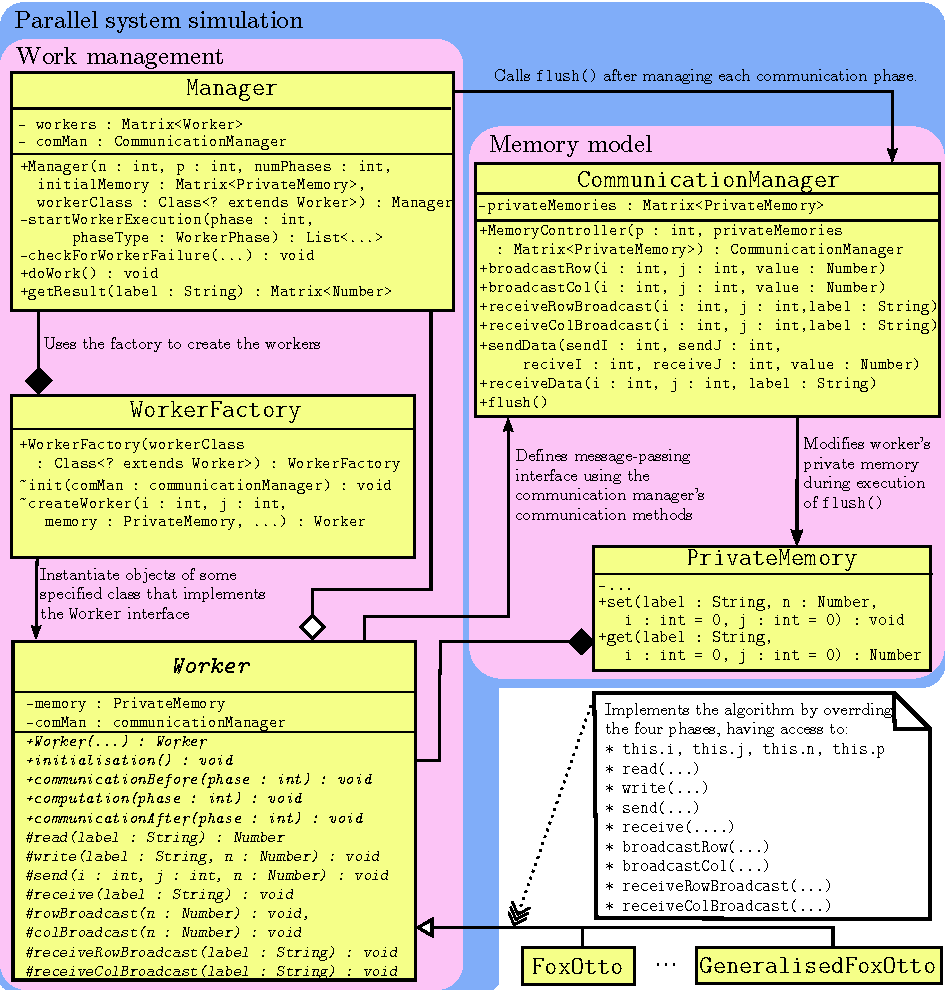
\includegraphics[scale=1]{figs/parallel-system-simulation.pdf}
\end{center}
\caption[Overview of the components of the parallel system simulator]{
    An overview of the main
    components of the simulator and how they interact. The \texttt{Manager}
    constructs the specified number of \texttt{Worker}s based on some provided
    subtype, for example \texttt{FoxOtto}, using a \texttt{WorkerFactory}. When
    \texttt{doWork()} is called, it will then run the \texttt{Worker}s through all
    of their communication- and computation-phases, and \texttt{flush()} the
    effects of their communication after each phase, which is done using the
    \texttt{CommunicationManager}. The \texttt{Worker} is an abstract class
    and provides a simple yet expressive interface for specifying
    parallel algorithms: The methods in cursive-bold are \texttt{abstract}, and
    must be overridden, but the rest of the methods can be used as is.
}
\label{fig:parallel-system-overview}
\end{figure}


\subsection{Memory model}%
\label{sub:Memory model}

% Explains string label access
To make memory access simple, we use string labels.
A \ac{PE} can then for example store a value
at location \texttt{"A"} and then retrieve it with the same label later.
Additionally, for \acp{PE} handling a non-$1\times 1$-submatrix, the
local memory is arranged in a \texttt{Matrix}
where the \ac{PE} can for example store
values at location \texttt{(1,4,"A")} to associate it with an intermediate
result $C_{1,4}$.

% Communication
To send point-to-point messages, both
the sender and recipient must call \texttt{sendData} and \texttt{receiveData},
respectively. The \texttt{receiveData(i, j, label)} method does not return a
value, but instead modifies the recipient's memory at location \texttt{label},
but this change does not happen until
\texttt{CommunicationManager::flush()} is called. When sending data with
\texttt{sendData}, \texttt{broadcastCol} or \texttt{broadcastRow}, the data
is buffered in the \texttt{CommunicationManager}. When \texttt{flush} is called,
all the buffered messages are matched up with corresponding calls
to \texttt{receiveData}, and the private memories of the recipients are
modified by the \texttt{CommunicationManager}. To prevent race conditions when
buffering data, fine-grained locking mechanisms are used within the
\texttt{CommunicationManager}.
An obvious alternative to this approach is making the \texttt{receiveData} method
return the number received, which can be done by putting the recipient
\texttt{Worker} to sleep until data has been received. Compared with this
approach, my approach allows cleanly separating computation and communication.
This, as we will see in the following subsection, gives many benefits.


% Work management points:
% * Diagram of how work is simulated in parallel fashion, 8 blocks at a time
% * Use Java's executor service to avoid thread management overhead
% * Briefly remind about interace, and communication method using one object
% * Manager explain, from construction, to how doWork works, to getResult, also
%   allowing reuse of workers, which is nice ...
% * Worker factory
%   * Use of reflection, so can allow arbitrary description to be passed and
%     can still
%     crete the new worker objects that can be managed
\subsection{Work management}%
\label{sub:Work management}

After describing an algorithm through the \texttt{Worker} interface, the
programmer sets up simulated execution with the \texttt{Manager}. They
specify the number of \acp{PE}, the problem size, the number of computation
iterations and the input. When \texttt{Manager::doWork} is called, execution is
simulated and the output can be retrieved with \texttt{getResult(label)}.

The work done by each simulated \ac{PE} is specified in phases, as seen in the
\texttt{Worker} interface in \cref{fig:parallel-system-overview}.
If we consider a single \ac{PE} in isolation, the order of these phases
is described in \cref{alg:execution-order}.
However, the work management is not that simple because
the \acp{PE} interact during communication phases. As we saw in the previous
subsection, the sent messages are put in a buffer and are not received until
\texttt{CommunicationManager::flush} is called. Therefore, if worker $i$ sends
a message to worker $j$ in their $n$th phase, the execution order dependency is
\begin{equation}\label{eq:data-dependency}
    \textrm{phase } n \textrm{ of } \textrm{worker}_i  \rightarrow \texttt{flush}
    \rightarrow \textrm{phase } n+1 \textrm{ of } \textrm{worker}_j.
\end{equation}
These constraints are satisfied by running all the
workers through one phase before moving onto the next phase, as visualised in
\cref{fig:work-management-blocks}. This execution pattern also allows
exploiting parallelism on the host machine for efficiency.

\begin{wrapfigure}{l}{0.53\textwidth}
\begin{minipage}{0.53\textwidth}
\begin{algorithm}[H]
    \caption{Execution of PE($i,j$)}%
    \label{alg:execution-order}

    $\texttt{worker.initialisation()}$\;

% \SetKwComment{Comment}{/* }{ */}
\For{$l = 0 \dots \textrm{number of iterations} -1$}{
    \texttt{worker.communicationBefore($l$)}

    \texttt{worker.computation($l$)}

    \texttt{worker.communicationAfter($l$)}

}
\end{algorithm}
\end{minipage}
\end{wrapfigure}

% TODO next jk work from here:
% * Move memory model above this one
% * make paragraph about why made design decision of splitting up into phases...
% * change up diagram on the blocks...
Splitting the work into phases has many benefits.
When investigating
the different algorithms, as well as possible extension like parallel
Floyd-Warshall, I noticed a clear distinction between computation
and communication. Enforcing a separation between the phases would therefore
not reduce the expressiveness. Instead, it allowed representing each phase
as an independent \texttt{Callable} task, which has many benefits.
Firstly, workers can be managed with
higher-level constructs like a Java \texttt{ExecutorService} instead of
having a Java \texttt{Thread} for each one.
This prevents the \ac{JVM} from creating more threads than what the host
computer can efficiently manage\footnote{
    This number is configurable, but since my Laptop
    can execute 8 threads simultaneously, I used this value.
} as the threads are reused for new computation, as shown in
\cref{fig:work-management-blocks}. As a result, we avoid a lot of the overhead
associated with
Java's \texttt{Thread} \acs{API}. Another benefit is implicit synchronisation.
Because of the data dependencies in \cref{eq:data-dependency}, we do not
need synchronisation primitives within the communication methods of each
\texttt{Worker}. Instead, synchronisation and correct execution order
is achieved through the scheduling of the work, as seen in
\cref{fig:work-management-blocks}.  The
third benefit of using work phases is allowing repeated execution of the same
work, which gives a more accurate computation time estimates.
% TODO: mention additional benefit: Easy to handle exceptions thrown by workers
%       and report them back to the caller while cleanly stopping all threads,
%       which makes development of the algortihms a lot easier, because can e.g.
%       see if receive's and send's are mismatched

% TODO: alternative diagram:
%   very small blocks with different colours, and the colours indicate whether it's
%   initilisatin, comBefore, compu, etc., and text inside is just e.g. "(0,0)"...
\begin{figure}
\begin{center}
    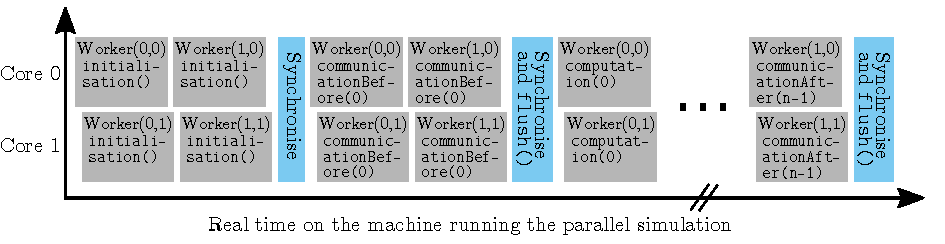
\includegraphics[scale=1]{figs/work-management-blocks.pdf}
\end{center}
\caption[Execution order when managing worker phases]{Example of multithreading when simulating 4 \acp{PE} on a host computer with 2 cores.}
\label{fig:work-management-blocks}
\end{figure}

The \texttt{WorkerFactory} uses Java's reflection \acs{API} to create instances of
any implementation of the \texttt{\textit{Worker}} interface. When constructing
this factory, the programmer provides a \texttt{Class} object of the
\texttt{FoxOtto} implementation, for example.
The factory can then infer the appropriate constructor
at runtime and create $p^2$ \texttt{FoxOtto}-workers, without needing
a dedicated Fox-Otto worker factory. This simplifies the interface
as implementing a \texttt{\textit{Worker}} is everything needed to
add a new parallel algorithm.

\subsection{Estimating computation and communication times}%
\label{sub:Estimating computation and communication times}

Even if we are using a simulator, we want the execution time measurements to
be as realistic as possible. This is achieved by measuring computation time
directly and using a communication model proposed by \citeauthor{hockney} for
message-passing \cite{hockney}. I first cover the theory and ideas behind
how the measurements are done, and then go into detail on how this
is implemented in the \texttt{timingAnalysis} package.

% The points to introduce this sub section with are:
% * Diagram of how communication causes stalls, counted as comTime:
%   * Split up phases into the 3 things, and can use arrow to indicate which PE
%     is sending to what, and assumption on if send-before, no delay to start
%     next phase...
% * What is measured as computation time
% * The equation for estimating communication, latency + bandwitdh * w, and
%   the assumptions made behind this

% TODO: Cite this \cite{hockney}, for details on $\alpha + w \cdot (n^2/p^2) \cdot \beta$

% TODO here: First, create the above diagram and write some stuff on
%      it, then the next task is creating a signpost introduction
%      paragraph just for this subsection, where say "first create the
%      model for communication, then go into how it's implemented, and
%      some clver tricks used to make it more accurate...."

\subsubsection{Measuring computation time}%
\label{ssub:Measuring computation time}


We can measure the computation time directly. By taking the difference
between the CPU time before and after the computation phase, we get a measure
for how long the phase was. We also want to minimize the
effects of running the code in a simulated environment. Compared to a real
parallel system, where there is dedicated processor and private memory for
each \ac{PE}, the memory and processing power on the host machine is
shared between all the simulated workers
and various background processes. This can cause unwanted effects such as
unexpected cache misses, due to other \acp{PE}' phases being simulated between
the execution phases of a particular \ac{PE}. Other effects include background
processes temporarily using a high \ac{CPU} load. To mitigate all this,
we want to repeat each phase several times and average their computation time.

\subsubsection{Mathematical model for communication}%
\label{ssub:Mathematical model for communication}

\begin{wrapfigure}{r}{.5\textwidth}
    \centering
    \fontsize{10pt}{10pt}
    \vspace{-10pt}
    \import{figs/}{communication-model.pdf_tex}%
    \vspace{-10pt}
    \caption[Demonstration of communication model through a simple
    example]{Example execution of three \acp{PE}, where simulated time is
        reconstructed with 
    \cref{eq:communication}. The ``$\delta t$''s are the time it takes to
    send a message, as defined in \cref{eq:send-time}.}%
    \label{fig:communication-model}
\end{wrapfigure}

The communication time is estimated with a theoretical model. The time it takes
to send a $s$-byte message can be modelled with $t=\alpha+\beta\cdot s$, which
is a model that has been previously used to estimate communication time
on parallel hardware \cite{hockney}.
To simplify the model, I assume that the constants $\alpha$ and $\beta$ are fixed
for all broadcast and point-to-point links. Incorporating our interconnect topology, if the
shortest distance between two \ac{PE}-nodes $i$ and $j$ is $\delta(i,j)$, then the time
it takes to send a message $m$ from node $i$ to $j$ is
\begin{equation}%
\label{eq:send-time}
    t(i,j,m) \triangleq
    \delta(i,j) \cdot (\alpha + \beta \cdot \textrm{size}(m)).
\end{equation}
Since each \ac{PE} executes independently, if recipient $j$ awaits data from
sender $i$ at some point in time, but the sender has not reached the appropriate
communication phase by then, the recipient must stall until $i$ is ready
and has sent the data. An example of this is shown when $PE_1$ sends a message
to $PE_2$ in \cref{fig:communication-model}.
To model this, let $T^{(n)}_i$ be the simulated time at
which \ac{PE} $i$ starts executing phase $n$. I make the simplifying assumption
that if the recipient has received all the data it expected by the time it reaches
the corresponding communication phase, it can immediately start the next phase
after sending off the data it needs to send. This happens for $PE_3$ in
\cref{fig:communication-model}. With this in mind, if \ac{PE}
$i$ is receiving data from a set of sender-\acp{PE}, $S$, and sending data to
a set of receivers, $R$, at communication phase $n$, which starts at time
$T^{(n)}_i$, then the next phase starts at
\begin{equation}%
\label{eq:communication}
    T^{(n+1)}_i = \max\left(
        \overbrace{T^{(n)}_i + \sum_{(j,m) \in R} t(i,j,m)}
        ^{\textrm{All necessary data has already arrived}}
    , \underbrace{\max_{(j,m) \in S} \left(T^{(n)}_j + t(j,i,m)\right)}
    _{\textrm{PE } i \textrm{ must stall until data has arrived}}
\right).
\end{equation}

\subsubsection{The \texttt{timingAnalysis} package}

The functionality for measuring the computation time of each \ac{PE} and
estimating the communication time required for message-passing is implemented
using the \textit{decorator} pattern, where an overview of the components
is shown in \cref{fig:timing-analysis-overview}. This pattern made implementation
more modular, allowing the core parts of the simulator to be developed before
timing measurements were added.

% TODO: blue background for what is part of the package....
% TODO: refactor Topology into this package, and include in diagram
\begin{figure}
\begin{center}
    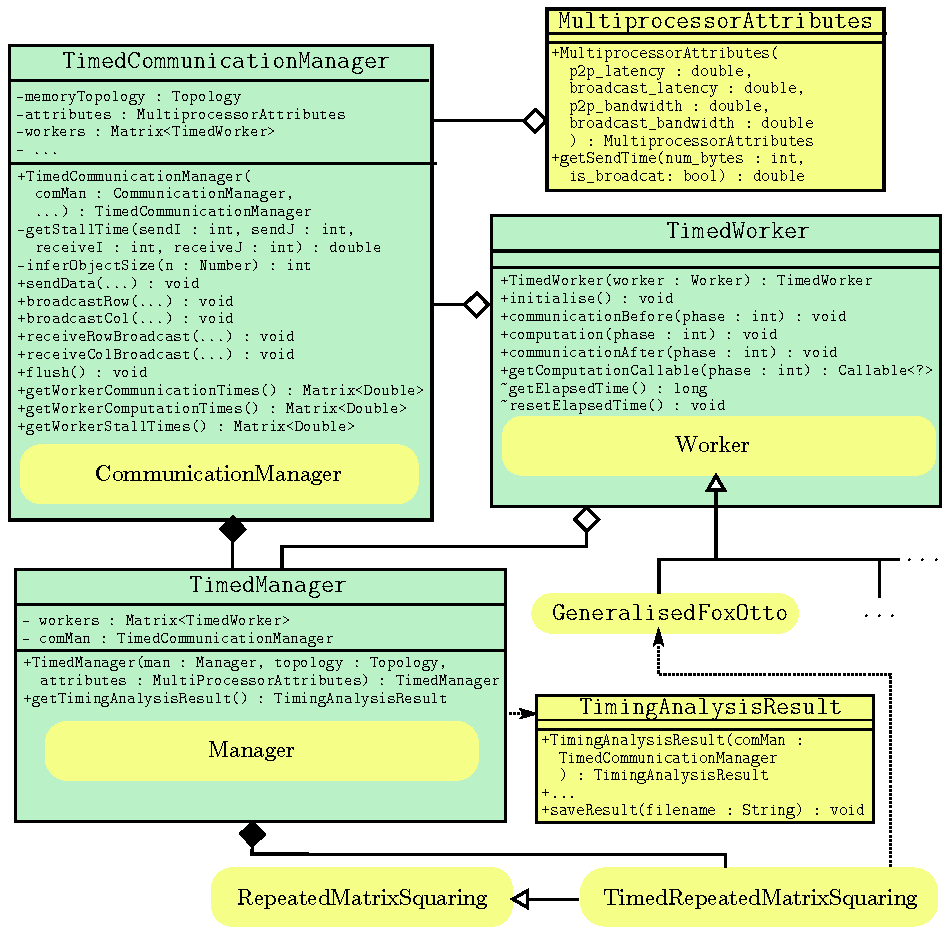
\includegraphics[scale=1]{figs/timing-analysis-overview.pdf}
\end{center}
\caption[An overview of the components in the \texttt{timingAnalysis} package]{An overview of the components of the \texttt{timingAnalysis} package.
Note that the \texttt{GeneralisedFoxOtto} and the \texttt{MatSquare}
classes are not part of this package. Additionally, the green class diagrams with
a yellow class inside it are short-hands for the decorator-pattern: The green
classes extend the base class, shown in yellow, and contains a reference
to it that is used to perform the original functionality in overridden methods
in addition to the timing analysis behaviour.}
\label{fig:timing-analysis-overview}
\end{figure}

% To explain:
% * In multiprocessorAttributes, can specify constants to use (ref equations)
% * These are used when computing message passing time in TimedComMan
% * In that class, maintain a matrix of the simulated real-time of all the \acp{PE}
%     and at each \texttt{flush()}, we update these based on stalling required
%     by the senders (as explained above...)
% * when the send or broadcast methods are called, we keep count of the number of
%   bytes sent, reset on flush, combine all in same packet possible, so programmer
%   don't need to worry about this. After this, do original functionality by
%   using held reference
% * In TimedManager, we decorate all the workers by constructing TimedWorker on them,
%   and we replace the Manager's existing \texttt{Matrix<Worker>} with these
%   using dynamic dispatch. TM also decorates the ComMan from the original Manager
% * In the TimedWorker, we use Java's \texttt{ThreadMXBean} to find the CPU time
%   each Worker spend on the CPU while running their \texttt{computation(phase :
%   int)} We also use a clever trick to minimize other effects, repeat computation
%   and take their average, not in cache, disable writes during this, so always
%   same branch, etc.

The \texttt{MultiprocessorAttributes} class is used to store what constants we
assume for the message-passing latency and bandwidth, $\alpha$ and $\beta$,
both for point-to-point messages and for broadcasting. We also implement the
$\delta$ function using the \texttt{Topology} interface. Together, these two
classes implement function $t$ in  \cref{eq:send-time}.

\begin{wrapfigure}{l}{0.45\textwidth}
    \begin{minipage}{0.45\textwidth}
        \begin{algorithm}[H]
            \caption{Measuring computation time in \texttt{TimedWorker}}%
            \label{alg:timed-worker}
            \KwData{Phase number $l$, \textit{num.~repeats}}
            \KwResult{Computation time $t$}

            \SetKwComment{Comment}{/* }{ */}

            % \Comment*[l]{Set worker to read only}
            \tcc{Enable read-only}

            \texttt{computation($l$)}\;

            $t_0 \gets \textit{current time }$\;

            \For{$i = 0 \dots \textrm{num. repeats} - 1$}{
                \texttt{computation($l$)}\;
            }

            $t \gets \frac{\textit{current time } -\,t_0}{\textit{num.
            repeats}}$

            \tcc{Disable read-only}

            \texttt{computation($l$)}\;
        \end{algorithm}
    \end{minipage}
    \vspace{-20pt}
\end{wrapfigure}

Most of the functionality for simulating execution time is found in
\texttt{TimedCommunicationManager}. Here, we maintain a matrix of the simulated
times of each \ac{PE}, with entries $(i,j)$ initially corresponding to times
$T^{(0)}_{(i,j)}$.
These entries are then updated whenever we advance from phase $(n)$ to phase
$(n+1)$, with different rules for the phase type.
For computation phases, we simply increment the time with
the measurement from the \texttt{TimedWorker}. For the communication phases,
we use the formula in \cref{eq:communication}, where the sets
$S$ and $R$ are constructed by tracking calls to \texttt{sendData},
\texttt{broadcastRow}, \texttt{receiveData}, etc.
We also only evaluate this formula when executing
the decorated \texttt{flush()} method after each communication phase.

In \texttt{TimedWorker}, we use a clever trick to get more accurate measures
for the computation time, as shown in \cref{alg:timed-worker}. The read-only
mode makes all side-effects of call to \texttt{Worker::store} be ignored.
This is necessary to ensure the computation always follows the same control
flow.  By running the unit of computation once before starting the timing,
the effects of cache misses are minimized as the used data will be in cache by
the time we get to the first timed \texttt{computation($l$)}. We also do several
runs and average these to minimize the effect of background processes running
on the host machine. I also want to emphasize that these tricks were only possible
because we separated computation and communication into phases when managing work.

% Points to write in some last paragraph on why this good idea:
% * By seperating the timing functionality, we make implementation easier and
%   modularise further. When timing the program complete seperate task, so first
%   focus on simulating processor, then focus on how to time this simulation. The
%   distinction between SIMD and MIMD will also just be present here, so could
%   for instance extend further with new decorator for SIMD
% * Also follow principle of each class doing one thing, so additional functionality
%   for e.g. repeated execution not mixed with the standard worker behaivour
% * The interaction between the components above are not all explicitly redone in
%   the decorators, but are instead present from the components underneath. For
%   instance manager, just decorates all the workers the manager already have
%   created with the WorkerFactory
% * How MIMD works, the stalling time etc., explained with a diagram...

% Components:
% * Topology
% * MultiprocessorAttributes
% * TimedManager
% * TimedRepeatedMatrixSquaring
% * TimedWorker
% * TimingAnalysisCommunicationManager
% * TimingAnalysisResult

% }}}

% APSP via repeated matrix-squaring
% * Can abbriviate as MatSquare or something
% * Start with top-down explanation, what happens when do A^2 and same for pred. matrix
% * Then explain the driver code, why this number of iterations etc.
% * Then explain generalized fox otto algorithm, noting special case for pred. matrix
% * Explain FoxOtto (explain predecessor functionality and edge-case,
%   generalized version, pseudo-code, diagram of memory movement can go in preparation)
% * Explain driver code, and its complexity?
% * As explain, also use a simple graph as an example, going through as you do the
%   general explanation
% APSP via repeated matrix-squaring {{{
\section{APSP via repeated matrix-squaring}%
\label{sec:APSP via repeated matrix-squaring}

% TODO: Set up more sign-posts here, add introrudction paragraph, followed by notation paragraph, where also say what $p$, $n$ is, etc., and how we pad the input. Then read through again and make sure whole of algorithm, referecning pseudo-code mroe throughly, comes through

We will now look at the \emph{\acl{MatSquare}} algorithm, which I will
abbreviate as \emph{\acs{MatSquare}}. I consider the generalised version of
the algorithm, which can handle any combination of $n$ and $p$.
However, before describing its execution,
I introduce some notation, and explain how the graph's adjacency matrix
is used to find shortest paths by using an operation called
the  \textit{distance product}.
We then consider the  predecessor matrix,
and how it is used to reconstruct paths. When introducing the algorithm
for finding the distance- and predecessor matrix, which is implemented in
\texttt{MatSquare.java}, I will look aside from how
the matrix-multiplication procedure is implemented, only focusing on
its desired semantics. Afterwards, I describe the parallel implementation of the
procedure, which is found in \texttt{GeneralisedFoxOtto.java},
and emphasize how it fulfils the semantics assumed.

\subsubsection{Notation}%
\label{ssub:Notation}

\begin{wrapfigure}{r}{0.20\textwidth}
    \centering
    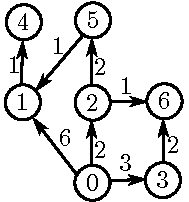
\includegraphics[scale=1]{figs/example-apsp-graph.pdf}
    \caption{A directed graph with 7 vertices.}%
    \label{fig:example-graph}
\end{wrapfigure}

Before getting to the description of the algorithm, we must go through
the notation I will be using. The parallel system has $p^2$ \acp{PE}, laid out
in a square lattice of size $p \times p$. We are solving \ac{APSP} for a graph
with $n$ vertices, so the input is a $n \times n$ adjacency matrix.
Before executing the algorithm, the adjacency matrix has been split up into
submatrices and been distributed evenly among the \acp{PE}. If $p$ does not
divide $n$, we pad the adjacency matrix such that each \ac{PE} receives
a submatrix of size $\lceil n / p \rceil \times \lceil n / p \rceil$. We refer
to the height and width of this submatrix as the \textit{submatrix size},
abbreviated $n'$. The padding happens by adding $\lceil n/p\rceil\cdot p-n$
vertices with no edges to the graph $G$. From here on, we will let $n$ be the
number of vertices in this padded graph, and the adjacency matrix $A$ will also
include inserted empty nodes. The goal of the algorithm is finding the distance-
and predecessor matrix.

\begin{definition}
    A distance matrix $M_{dist}$ is a  $n \times n$ matrix, whose $(i,j)$
    entry is the length of a shortest path $i \rightsquigarrow j$ in graph
    $G=(V,E,w)$. If there is not such path, the entry is $\infty$.
\end{definition}

\begin{definition}
    A predecessor matrix $M_{pred}$ is a $n \times n$ matrix, whose $(i,j)$
    entry is the immediate prior node to $j$ in a shortest path $i
    \rightsquigarrow j$ in graph $G=(V,E,w)$. If there is no such path, the
    entry is $j$.
\end{definition}

We also refer to $M_{dist}^{(x)}$ and $M_{pred}^{(x)}$ as the corresponding
matrices, but only considering paths of \textit{at most} $x$ edges. This then
gives that $M_{dist}^{(n)}$ and $M_{pred}^{(n)}$ are distance and predecessor
matrices, respectively\footnote{As long as the graph $G$ does not have negative
cycles}.


% From here, add more references to pseudo-code. We want to take the reader
%  through the whole algorithm so they fully understand it!

\subsubsection{The \ac{MatSquare} algorithm}%
\label{ssub:The algorithm}


This algorithm computes
the distance- and predecessor matrix. 
Let  $A$ be the adjacency matrix for graph $G$.
We want to add self-loops to each vertex, by setting
$A_{i,i} \leftarrow 0$ for each $0 \leq i < n$, because
it allows repeated distance products to capture shorter paths. For example,
if  $A$ is the adjacency matrix for the graph in \cref{fig:example-graph},
$A^4_{0,1}$ would be the length of the path $1 \xrightarrow{2} 2
\xrightarrow{0} 2 \xrightarrow{2} 5 \xrightarrow{1} 1$, which in practice just
contains 3 edges.  We notice that this modified adjacency matrix fits the
definition of $M_{dist}^{(1)}$. Additionally, computing the
distance product between two matrices $M_{dist}^{(x)}$ and $M_{dist}^{(y)}$ gives
a matrix $M_{dist}^{(x+y)}$ containing distances of shortest paths of length at most
$x+y$. As such, one way to compute the distance matrix is
\begin{equation}
    M_{dist}=M_{dist}^{(n)}=
    \underbrace{M_{dist}^{(1)} \otimes \cdots \otimes M^{(1)}_{dist}}_{n-1 \textrm{ times}}
    =
    \underbrace{A \otimes \cdots \otimes A}_{n-1 \textrm{ times}}
\end{equation}%
%
\begin{wrapfigure}{r}{0.55\textwidth}
    \begin{minipage}{0.55\textwidth}
        \begin{algorithm}[H]
            \caption{MatSquare}%
            \label{alg:matsquare}
            \SetKwInOut{Input}{Input}
            \SetKwInOut{Result}{Result}

            \Input{Adjacency matrix $A$}
            \Result{Distance matrix $M_{dist}$, Predecessor matrix $M_{pred}$}

            $M_{dist} \gets A$\;

            $M_{pred} \gets n \times n \textrm{ matrix}$\;

            \For{$(i,j) \in V^2$}{
                $M_{pred}[i,j] \gets i \textbf{ if } A_{i,j} < \infty
                \textbf{ else } j$\;
            }

            \tcp{Repeated squaring}
            \For{$x = 1 \dots \lceil \log_2 n \rceil$}{
                $M_{dist} \gets M_{dist} \otimes M_{dist}$\;
                $W \gets \textrm{witness matrix for above } \otimes$\;
                \For{$(i,j)\in V^2$}{
                    \If{$W_{i,j} \neq j$}{
                        $M_{pred}[i,j] \gets M_{pred}[W_{i,j}, j]$\;
                    }
                }
            }
        \end{algorithm}
        \vspace{-15pt}
    \end{minipage}
\end{wrapfigure}%
However, we can reduce the number of distance product matrix multiplications
from $\Theta(n)$ to $\Theta(\log n)$ by squaring $A$ $\lceil \log n \rceil$
times, which is what happens in the \texttt{for}-loop in \autoref{alg:matsquare}.
With this transformation, we may overshoot by finding $M_{dist}^{(n')}$ for
$n'>n$, but this will be the same matrix because all the shortest paths cannot
be of length longer than $n$.

\paragraph{Reconstructing paths}%
\label{par:Reconstructing paths}

We have now described how to compute the length of the shortest paths, but we
would also like to reconstruct the list of nodes that make up these paths.
When computing 
$M_{i,j}\leftarrow\min_{0 \leq k < n}(M_{i,k}+M_{k,j})$ as part of the distance
product $\otimes$, the operation corresponds to finding the optimal intermediate node $k$ such that $i \rightsquigarrow k \rightsquigarrow j$ is the shortest path
from $i$ to $j$. If we already know the predecessor of $j$ in the path
$k \rightsquigarrow j$, then the predecessor of $j$ in path
$i \rightsquigarrow k \rightsquigarrow j$ must be same. This allows us to
correctly update the predecessor matrix after each distance product.
Formally, we call these intermediate nodes for \textit{witnesses} \cite{stanford}, where
\begin{definition}
    A witness matrix $W$ for a distance product $M \otimes M'$
    is a $n \times n$ matrix, whose entries $(i,j)$ are witnesses
    \begin{equation}
        w_{i,j}=\argmin_{0 \leq k < n} ( M_{i,k} + M'_{k,j}).
    \end{equation}
\end{definition}
These predecessor updates happen on lines 8--13 in \autoref{alg:matsquare}.
We also note that the witness $k$ may be equal to $j$, in which case the path
$k \rightsquigarrow j$ is a self-loop. This will obstruct the path reconstruction
algorithm, so we want to keep the old predecessor value
in those cases, hence the \texttt{if}-statement on line 10.

The algorithm to reconstruct  the paths is simple once we have computed
the predecessor matrix $M_{pred}$. Given a query $i \rightsquigarrow j$, we
start with a list of vertices $[j]$, and repeatedly prepend the predecessor of the
first vertex. We stop when we arrive at $i$ or find a self-loop. In the latter
case, the vertices are not connected. This is also why we initialise the
predecessor entries $M_{pred}^{(x)}[i,j]$ to $j$ if there
are no paths $i \rightsquigarrow j$ of length $x$.  An example of this algorithm
is shown in \cref{sec:path-reconstruction}.

% TODO: read through all of the above, and add signposts including: "We
% implement this in driver code, and use manager to compute \otimes, distance
% product, and don't directly compute witness matrix, but same semantics....

% Define pred.matrix, distance matrix, after squaring $x$ times, why log n ceil
% squarings necessary. Explain that create Manager/Worker that implement this
% operation, so in driver code, we simply (1) prepare initial memory (2) run
% the PEs ceil times, and mem Movement such a way, no need to reset memory
% because if dist, pred in memory, assigns to "A", "B" and "P"...
% ^ could have pseuocode for this part?

\subsubsection{Parallelising MatSquare with FoxOtto}%
\label{ssub:Parallelising MatSquare with FoxOtto}


We will now look at how to parallelise the matrix multiplication step and
associated assignments in lines 6--14 of \autoref{alg:matsquare}. I describe a
parallel algorithm to perform the operations of a single iteration of the
\texttt{for}-loop on lines 7--13 in \autoref{alg:matsquare}, and this procedure will
be executed $\lceil \log_2 n \rceil$ times. In each iteration, $p^2$ \acp{PE}
execute \autoref{alg:foxOtto} in parallel. To simplify the explanation, we
consider what happens in the \texttt{for}-loop of \autoref{alg:matsquare}
using slightly different
notation: Let $A$ be the left matrix of the distance product and $B$ be the
right matrix, such that both matrices are equal to $M_{dist}$ at line 7.
We also let $P$ be the predecessor matrix $M_{pred}$.
We think of these three matrices as the input.
After the parallel procedure, the distance product and the predecessor matrix---%
the output---%
should be stored in $M_{dist}$ and $M_{pred}$, respectively,
just like in \autoref{alg:matsquare}. On following executions, $M_{dist}$ and
$M_{pred}$ are fed back into the procedure as inputs $A,B$ and $P$.

\begin{algorithm}[htp]
    \caption{Generalised Fox-Otto execution at processing element $p_{i,j}$}%
    \label{alg:foxOtto}
    \SetKwInOut{Parameter}{Parameter}
    \SetKwInOut{Data}{Data}
    \SetKwInOut{Result}{Result}
    \Data{$A',B',P'$}
    \Parameter{problem size $n$, PE grid size $p$, subMatrixSize $n'=\lceil n/p\rceil$,}
    \Result{$M_{dist}', M_{pred}'$}

    \tcpp{ ** Initialisation phase **}
    $A_{const}' \leftarrow A'$\;
    $M_{dist}' \gets n' \times n' \textrm{ matrix}$\;
    $M_{pred}' \gets n' \times n' \textrm{ matrix}$\;
    \For{$0 \leq i_2,j_2 < n'$}{
        $M_{pred}'[i_2,j_2] \gets j$\;
        $M_{dist}'[i_2,j_2] \gets \infty$\;
    }

    \For{phase number $l = 0$ to $p-1$}{

        \tcpp{ ** CommunicationBefore phase $l$ **}

        \If{$j = (i + l) \mod p$}{
            \tcp{Received as a submatrix $A'$}
            \texttt{broadcastRow(}$A_{const}'$\texttt{)}\;
        }
        \tcpp{ ** Computation phase $l$ **}
        \For{$0 \leq i_2,j_2 < n'$}{
            \tcp{We start with $m$ s.t. $k=i'$ at $l=0$, which causes shorter}
            \tcp{paths from the previous squaring to be considered first.}
            \tcp{This is necessary to get the predecessor right.}
            \For{$m=i_2,i_2+1, \dots n'-1, 0, 1, \dots, i_2-1$}{


                \tcpp{In this iteration, we compute A[i', k] + B[k, j'], where}
                $k \gets (n' \cdot (i+l) + m) \mod n$\;
                $i' \gets i \cdot n' + i_2$\;
                $j' \gets j \cdot n' + j_2$\;
                \tcpp{Distance product}
                $d_{new} \gets A'[i_2,m] + B'[m,j_2]$\;

                \If{$d_{new} < M_{dist}'[i_2,j_2]$}{
                    $M_{dist}'[i_2,j_2] \gets d_{new}$\;
                    \tcp{If $k=j'$, the path $k \rightarrow j'$ will be a self-loop, so}
                    \tcp{we should not update the predecessor}
                    \If{$k \neq j'$}{
                        \tcp{The cell $P'[m,j_2]$ holds $P_{k,j'}$}
                        $M_{pred}'[i_2,j_2] \gets P'[m,j_2]$\;
                    }
                }
            }
        }
        \tcpp{ ** ComunicationAfter phase $l$ **}
        \texttt{send(}$p+i-1 \mod p$\texttt{, }$j$\texttt{, }$B'$\texttt{)}\;
        \texttt{send(}$p+i-1 \mod p$\texttt{, }$j$\texttt{, }$P'$\texttt{)}\;
    }
    % (subMatrixSize * (i + l) + iter) % n !=
    %  subMatrixSize * j + j2
    %
    %  if not (j2 == iter
    %      and j == (i + l) mod n)
    %     update
\end{algorithm}

\begin{wrapfigure}{r}{0.42\textwidth}
    \vspace{-0pt}
    \centering
    \fontsize{7pt}{7pt}
    \vspace{-10pt}
    \import{figs/}{fox-otto-diagram.pdf_tex}%
    \caption{Message-passing pattern used in the Fox-Otto technique.}%
    \label{fig:fox}
    \vspace{-15pt}
\end{wrapfigure}

To parallelise the procedure, we distribute the input $A$, $B$, and $P$ 
evenly among the $p^2$ \acp{PE} by dividing them up into submatrices of size
$\lceil n / p \rceil \times \lceil n / p \rceil$. For example, if we use a
$2 \times 2$ lattice arrangement and distribute the adjacency matrix
of graph in \cref{fig:example-graph}, the \ac{PE} with id $(0,1)$ would receive
entries $[0\dots 3,4\dots 7]$ of matrices $A,B,P$.
It would also be
responsible for computing the submatrices $M_{dist}[0\dots 3, 4\dots 7]$ and
$M_{pred}[0\dots 3, 4\dots 7]$.
As submatrices of $A,B$ and $P$ are shifted around during communication,
I use the notation $A',B'$ and $P'$ to refer to submatrices the \ac{PE}
currently holds, but that might be moved around later. Also, $M_{dist}'$ and
$M_{pred}'$ refer to the submatrices a \ac{PE} is responsible for computing.

If we consider the computation of an entry $(i',j')$ in
the distance product, as defined in
\cref{eq:distanceProduct}, the order of the products
 $A_{i',j} \cdot B_{k,j'}$  does not matter because the $\min$-operator is
commutative. By first considering the data that is local to each \ac{PE} first,
and then considering other $k$s as data is shifted around, the \acp{PE} can
simultaneously perform minimisations without requiring more than
$O(\lceil n^2 / p^2 \rceil)$ memory.
 \citeauthor{fox} describe
a data movement technique for doing this \cite{fox}. As shown in
\cref{fig:fox}, this technique consists of broadcasting the submatrices of
$A$ along the rows before partially computing the $\min$. After computation,
the submatrices of $B$ are shifted upwards to the next \ac{PE}. This pattern
ensures that in the computation phases, all the \acp{PE} have access to
matching submatrices of $A$ and $B$. These communication
phases are implemented in lines 9--11 and 26--27 in \autoref{alg:foxOtto}.


% \begin{wrapfigure}{r}{0.36\textwidth} % at scale 1.0
\begin{wrapfigure}{r}{0.27\textwidth}
    \vspace{-20pt}
    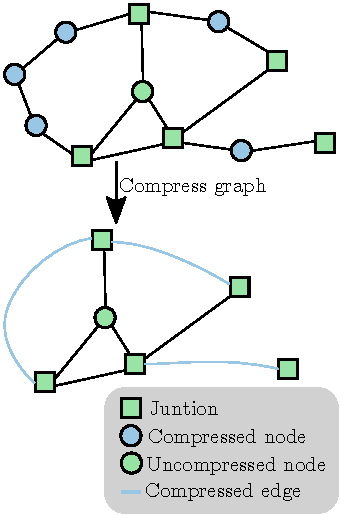
\includegraphics[scale=.8]{figs/compression-notation.pdf}
    \caption{Graph before and after compression.}%
    \label{fig:compression-notation}%
    \vspace{-20pt}
\end{wrapfigure}

Since each \ac{PE} $p_{i,j}$ is responsible for computing a $n'\times n'$
submatrix of $M_{dist}$ and $M_{pred}$, we have two \texttt{for}-loops on line
12 that iterate all the entries $(i_2,j_2)$ in these submatrices. In each of
these iterations, we loop through the $n'$ witnesses on line 13 and compare the
new distance term with the current minimum distance on lines 17--18 in accordance
with the definition of the distance product. 
We can ascertain ourselves that $A'[i_2,m]$ and $B'[m,j_2]$ contain matching elements of
the matrices $A$ and $B$ by working through the data movement pattern in
\cref{fig:fox}. In fact, it can be shown that on line 17, we are computing
$A[i',k] + B[k,j']$ with $i',j'$ and $k$ as defined on lines 14--16
(see \cref{sec:Proof of correct addition in generalised FoxOtto}).
Therefore, the witness will be $k$, which makes the predecessor update logic
on lines 20--22 equivalent to what is done in lines 11--13 in
\autoref{alg:matsquare}. 

% Conclusion where explain time complexity and memory complexity
% and relate this to $p$, and what complexity is then...

% Notes from reserach-and-planning diary:
% **Problem with generalized FoxOtto**:
% In the general version, we first started the multiplication by iterating from
% the top of the submatrix (see diagram in notes for $C_{10,6}$ for instance).
% However, this causes problems for the predecessor values because of the initial
% conditions. Consider the scenario for $C_{10,6}$ where want to compute path 10
% -> 10. Whenever we get to $k=10$, we would not assign predecessor because of
% exemption condition (which is necessary, otherwise we get other bugs). And at
% this point ($k=10$) we discover path of length 0. However, because of the
% generalization, we start with $k=8$ (ref. to diagram), so we find another path
% of longer length, and when we get to $k=10$, we optimize the path, but leave
% the predecessor as it was for the longer path because of the exemption
% condition. One fix is to save the initial "dist" and not use $\infty$ every
% time. Another option is making sure we start with $k=10$ when running algo i.e.
% being consistent with non-general version. That way, we immediately relax
% distance to 0 and keep the initial predecessor, this.j (or read("P") which is
% same thing). This is the option I went for, and is the reasoning behind the `m`
% loop and then modifying `iter`.
%
% * In `CountingMemoryController`, we assume
% that each PE only sends data to **one** other PE, but this is NOT CHECKED
% anywhere. However, it is enforced in underlying memory controller that each PE
% can only receive from **one** other PE, which is not equivilant, but in _most
% cases_ (all PE do the same thing) causes the above assumption to hold.

% TODO TODO: Compile list of all things about graphs, predecessors etc. that I
%            mention here, and put those in the preperation chapter!

% }}}

% Graph compression:
% * The algorithm for this, and explain all the edge cases, **with diagrams**
% * Also simple graph to use as an example
% * Also a section for the expected asymptotic speed-up referencing random graph generation
% Graph compression {{{
\section{Graph compression}%
\label{sec:Graph compression}

% Paragraph on motivation:
% * Table of number of 2-degree nodes in each graph dataset, and proportion
%   reduction, e.g. graph size reduced by 15 times
% * In general, road-networks are often very sparse
% Paragraph on how transformation works
% * Introduce notation
% * Example graph, showing how work
% Inverse transformation
% * Want to perform inverse transform as well, so extra book-keeping as compress
% * In `GraphCompressor`, which subclasses `APSPSolver`
% * Something about how nice this is, reduce computation requires, while as
%   powerful as solve the original problem as well
% Algorithm
% * Diagram of all the possible cases (look at code and `me` on how this done)
Most road networks are sparse, so many of the vertices will just
have two neighbours. This can be used to reduce the amount of computation
as there is only one path across a segment of two-degree nodes. In this section,
I present an algorithm for compressing segments of two-degree nodes into a single
edge. As we see in \cref{tab:size-reduction}, this can significantly
reduce the problem size of real-world road networks, especially the Californian
road network.

\begin{table}
    \centering
    \begin{tabular}{|c|c|c|c|}
        \hline
        \textbf{Road network} & \textbf{Nodes} &
        \textbf{2-degree nodes} & \textbf{Size reduction} \\
        \hline
        California          & 21048  & 19683  & $\times 15.4$ \\
        \hline
        San Francisco       & 174956 & 29627  & $\times 1.2$  \\
        \hline
        North America       & 175813 & 166687 & $\times19.3$ \\
        \hline
        City of San Joaquin & 18263  & 3760   & $\times1.26$ \\
        \hline
        City of Oldenburg   & 6105   & 3232   & $\times2.12$ \\
        \hline
    \end{tabular}%
    \caption{Possible size reduction by removing 2-degree nodes from different
    road networks}%
    \label{tab:size-reduction}
\end{table}

We compress the graph by removing all nodes with exactly two neighbours and
their edges. We refer to a contiguous sequence of such compressed
nodes as a \textit{(compressed) chain}, and compensate for its removal by
adding a new edge between the \textit{junctions} of the compressed chain,
as shown in \cref{fig:compression-notation}. The weight of the new edge
is the sum of the weight of the edges removed. We do this for all chains containing
at least one node of degree two. There are two edge-cases that may occur during
the compression. Firstly, if the two junctions are the same node, I let
a 2-degree vertex adjacent to the junction be the second junction.
This avoids introducing
more edge-cases in the path-reconstruction step later.
% TODO: rename Compressed edge -> compression edge, and make colour darker
Secondly, if we have a two-degree-node path $p \rightarrow n_1 \rightarrow \cdots
n_l \rightarrow q$ between two junctions $p$ and $q$, and there is an edge
$(p,q) \in E$, then the compressed graph will have two different edges
between $p$ and $q$. In this case, I only keep the edge with the lowest
weight, discarding the other.

To get any benefit from running some \ac{APSP} algorithm, like the
\ac{MatSquare} algorithm, on the compressed graph, we must be able to map path
queries for the original graph onto the compressed graph, and then
map back the result. To do this, extra bookkeeping during graph compression is
needed. For each compressed node, we store a map to its two junctions, the list of
vertices in the paths to the junctions, and the length of these paths. Additionally,
with each compressed chain of vertices, we store the list of compressed nodes.

\begin{figure}[htp]
    \begin{center}
        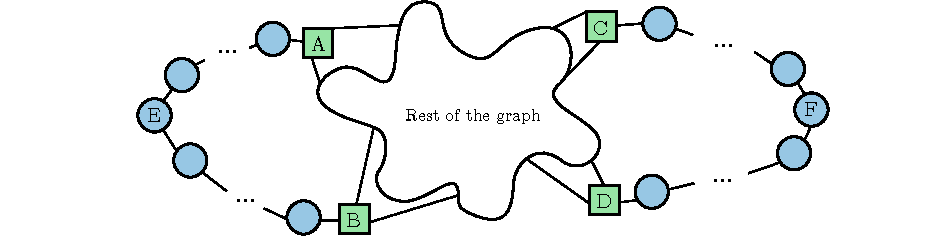
\includegraphics[scale=1]{figs/compression-diagram.pdf}
    \end{center}
    \caption[Visualisation of original graph before compression]{Without loss of generality, if the original graph has at least one
    node with degree 2, we can visualise  it like this.}
    \label{fig:compression-diagram}
\end{figure}

To answer an \ac{APSP} query $p \rightsquigarrow q$, and reconstruct its path,
consider the original graph in 
\cref{fig:compression-diagram}.
We have 5 cases, each of which gives different queries to the compressed graph:
\begin{enumerate}
    \item Nodes $p$ and $q$ are on the same compressed chain, in which case
        no queries are made. Instead, we compute the path using
        the list of vertices associated with the compressed chain vertices
        $p$ and $q$ were a part of.
        This case corresponds to $A=C$ and $B=D$, or some symmetric case, in
        \cref{fig:compression-diagram}.
    \item We have $p=E,q=F$. We compute the four paths,
        $p \rightsquigarrow \{A,B\} \rightsquigarrow \{C,D\} \rightsquigarrow q$,
        and use the shortest one. This gives four queries on the compressed graph.
    \item  We have $p\in \{A,B\},q=F$. We compute the two paths, one going
        through junction $C$ and the other through $D$. The queries on the
        compressed graph are $p \rightsquigarrow C$ and $p \rightsquigarrow D$.
    \item We have $p=E,q\in \{C,D\}$. This is symmetric to case (3).
    \item We have $p\in \{A,B\}, q\in \{C,D\}$. Both nodes are on the compressed
        graph, so we query $p \rightsquigarrow q$.
\end{enumerate}
For all of the above cases, we get back a path on the form:
\begin{equation}
    p\; \rsquigarrow{nodes just in original graph}{18}\;
    J_1 \;\rsquigarrow{nodes just in compressed graph}{20}\;
    J_2 \; \rsquigarrow{nodes just in original graph}{18}\; q,
\end{equation}
where any of the three subpaths may be empty. To map this back to a path in
the original graph, we must expand all the edges in the path $J_1 \rightsquigarrow J_2$ to a path in the original
graph. This is done by going through each edge, and swapping the compressed
chain out for the list of edges that were compressed.

% }}}

% Summary
% Summary {{{
\section{Summary}%
\label{sec:Summary1}

In this chapter, I explained the components implemented throughout the project.
I discussed the datasets used as input. Then I went into depth on how I
implemented a simulation of a parallel system, which met the requirements
outlined in \autoref{sec:Requirements analysis}. The
timing-estimation functionality exceeded what was initially proposed, and the
interface for writing parallel programs was very successful.  I then explained
the \ac{MatSquare} algorithm, by first considering a high-level overview of it,
followed by an in-depth description of how the computation was parallelised.
The \ac{MatSquare} algorithm described was a generalised version, which was one
of the extensions proposed.
Lastly, I looked at an optimisation that could significantly reduce the
computation time required for solving \ac{APSP} on sparse graphs. This was also
an extension.

% }}}



% vim: foldmethod=marker
